\documentclass{jarticle}
\usepackage{listings, jlisting}
\usepackage[dvipdfmx]{graphicx}
\usepackage{here}
\usepackage{geometry}
\usepackage{comment}
\usepackage{url}

\geometry{left=25mm,right=25mm,top=30mm,bottom=30mm}

\title{マーケティング科学期末レポート}
\author{1610285 酒井啓輔
\thanks{電気通信大学情報理工学域1類経営・社会情報学プログラム}}

\begin{document}
\begin{titlepage}
\maketitle
\thispagestyle{empty}
\end{titlepage}

\section{課題}
スマートフォンの市場について考える。
そのうち自分の使っているSHARPについてマーケティング戦略を策定する。

まず市場調査を行う。
データは後述するwebサイトから参照した。
集めたデータラベルは
\begin{itemize}
\item 最大クロック数
\item コア数
\item RAM
\item ROM
\item 重量
\item 画面解像度(縦・横)
\item 画面サイズ
\item 本体の厚さ
\item 非接触充電機能の有無
\item ワンセグ
\item OS
\item 価格
\item 外カメラ画素数
\item 内カメラ画素数
\item バッテリー容量
\item 販売台数
\end{itemize}
調べる企業は
\begin{itemize}
\item Apple
\item Sony
\item SHARP
\item SAMSUNG
\item Fujitsu
\item HUAWEI
\end{itemize}
それぞれハイエンド機種を代表として比較した。
機種は以下の通り
\begin{itemize}
\item iPhoneXR
\item Xperia XZ3
\item AQUOS R2
\item Galaxy Note9
\item arrows NX
\item HUAWEI P20 Pro
\end{itemize}

\section{重回帰分析を用いた市場の推定}
これらの値を重回帰分析を行うことで販売台数を目的変数とする重回帰式を求める。
重回帰分析にはsklearnを使用した。

\begin{lstlisting}[caption=重回帰分析, frame=single, language=python]
import pandas as pd
from sklearn import linear_model
import numpy as np

HEADER_ENGLISH = ('clock', 'core', 'RAM', 'ROM', 'Weight',
                'screen', 'height', 'width', 'depth',
                'wireless_charge', 'one_seg','ios', 
                'Android', 'value', 'out_camera', 
                'in_camera', 'battery', 'share'
                )
df = pd.read_csv('data.csv', encoding='shift-jis'
                , names = HEADER_ENGLISH
                , index_col = 0
                , skiprows = 1
                )
clf = linear_model.LinearRegression()

# 正規化して使用した
df_normalize = df.apply(lambda x:(x-np.mean(x))/(np.max(x)-np.min(x)))

# 正規化した結果iosと同じ値となったのでAndroidとcoreのカラムは消去した
df_expect_share = df_normalize.drop('share', axis = 1)
df_expect_share = df_expect_share.drop('Android', axis = 1)
df_expect_share = df_expect_share.drop('core', axis = 1)

Y = df_normalize['share']

# fitting
clf.fit(df_expect_share, Y)

print(pd.DataFrame({"Name":df_expect_share.columns
                   ,'Coefficients':clf.coef_ }))
        )

'''
               Name  Coefficients
0             clock      0.002580
1               RAM     -0.244887
2               ROM     -0.077489
3            Weight      0.104058
4            screen      0.121683
5            height      0.066245
6             width     -0.199049
7             depth     -0.080575
8   wireless_charge     -0.013213
9           one_seg     -0.142940
10              ios      0.329605
11            value     -0.044795
12       out_camera     -0.197650
13        in_camera     -0.074062
14          battery     -0.103846
'''
# 切片
print(clf.intercept_)
# -3.284491206674276e-17

# 寄与率
print(clf.score(df_expect_share, Y))
# 1.0
\end{lstlisting}
この変数のうち係数の絶対値の大きいios, RAM, out\_camera, widthを採用した。

この4つの変数を用いて推定した結果を可視化したものが以下である。
\begin{figure}[H]
	\centering
	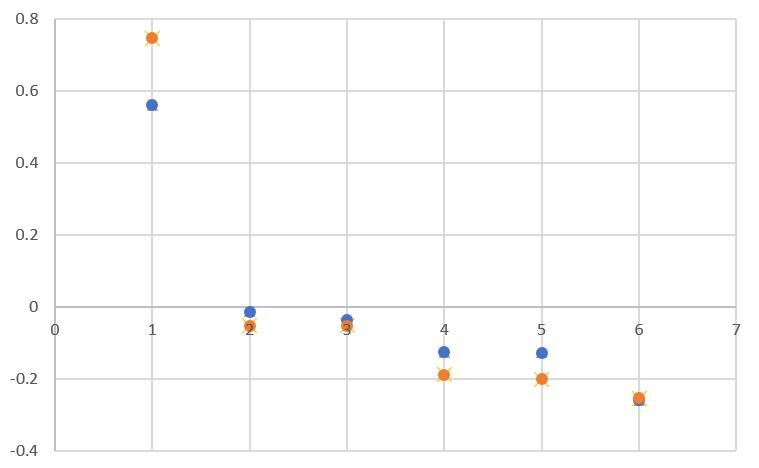
\includegraphics[width=15cm]{share_saigen.jpg}
	\caption{重回帰分析による近似値と実測値}
\end{figure}

\section{市場の作成}
今回考えるマーケティング戦略は各属性についてどのように広告費を振り分けると効率が良いかである。
今回ピックアップした4つの属性についてSHARPはどの属性を押し出して広告するのが効率的だろうか。

消費者数は1000
各消費者の重視度は平均を重回帰分析で求めた係数として重みづけた正規分布に従う乱数とした。
標準偏差は0.5で設定した。

\begin{lstlisting}[caption=市場の作成, frame=single, language=python]
import pandas as pd
import numpy as np

ios = np.random.normal(loc = 0.329605, scale = 0.5, size = 1000)
RAM = np.random.normal(loc = -0.244887, scale = 0.5, size = 1000)
out_camera = np.random.normal(loc = -0.19905, scale = 0.5, size = 1000)
width = np.random.normal(loc = -0.19765, scale = 0.5, size = 1000)

market = pd.DataFrame([ios, RAM, out_camera, width])

market.T.to_csv('market.csv')
\end{lstlisting}

同時に正規化した各製品の属性値を求めておく。
\begin{lstlisting}[caption=正規化した各製品の属性値, frame=single, language=python]
HEADER_ENGLISH = ('clock', 'core', 'RAM', 'ROM', 'Weight', 'screen',
                 'height', 'width', 'depth', 'wireless_charge',
                  'one_seg','ios', 'Android', 'value', 
                  'out_camera', 'in_camera', 'battery', 'share'
                                        )
product_data = pd.read_csv('data2.csv', encoding='shift-jis'
                , names = HEADER_ENGLISH
                , index_col = 0
                , skiprows = 1
                )

# 抽出
product_data = product_data.loc[:,['ios', 'RAM', 'out_camera', 'width']]

# 正規化
product_data = product_data.apply(lambda x: (x-np.mean(x))
          /(np.max(x) - np.min(x)))
          
'''
	ios	RAM	out_camera	width
iPhone XR	0.833333	-0.500000	-0.339286	-0.485348
Xperia XZ3	-0.166667	-0.166667	-0.082143	0.075092
AQUOS R2	-0.166667	-0.166667	0.039286	0.075092
Galaxy Note9	-0.166667	0.500000	-0.332143	0.075092
arrows NX	-0.166667	-0.166667	0.053571	0.514652
HUAWEI P20 Pro	-0.166667	0.500000	0.660714	-0.254579
'''
\end{lstlisting}

\section{広告効果の設定}
今回多属性モデルと広告の効果を以下の式とした。
$$U_j = \Sigma{(b_{ij}*e_i*m_{ij})}$$
\begin{itemize}
\item $b_{ij}$ 製品jの属性iの値
\item $e_i$ 顧客の属性iの重視度
\item $m_{ij}$ 製品jの属性値iの顧客の理解度
\end{itemize}

また理解度は広告費に基づく指数分布に従い
$$m_{ij} = 0.003^{\exp{(-0.04*a_{ij}})}$$
とした。
各社が持っている資金は200でSHARP以外の企業はどの属性値にも50ずつ広告費を投入する。

標準偏差を0.1として正規分布に従う乱数として各ユーザーごと製品ごと属性ごと決定した。

\begin{lstlisting}[caption=各製品の属性ごとの理解度, frame=single, language=python]
def ad_effect(money):
    return 0.003**np.exp(-0.04*money)
    
marketing = pd.DataFrame([[50, 50, 50, 50]
                          , [50, 50, 50, 50]
                          , [50, 50, 50, 50]
                          , [50, 50, 50, 50]
                          , [50, 50, 50, 50]
                          , [50, 50, 50, 50]
                          ]
                         , columns = ['ios', 'RAM', 'out_camera', 'width']
                         , index= ['Apple', 'Sony', 'SHARP', 
                                'SAMSUNG', 'Fujitsu', 'HUAWEI']
                        )

effect_of_marketing = []
for i, name in enumerate(marketing.index):
    for j, column in enumerate(marketing.columns):
        effect_of_marketing.append(np.random.normal(
        				loc = ad_effect(marketing.iloc[i, j])
                                       , scale = 0.1
                                       , size = 1000
                                       )
                  )
effect_of_marketing = np.array(effect_of_marketing)

pd.DataFrame(effect_of_marketing).T.to_csv("effect.csv")
\end{lstlisting}

\begin{figure}[H]
	\centering
	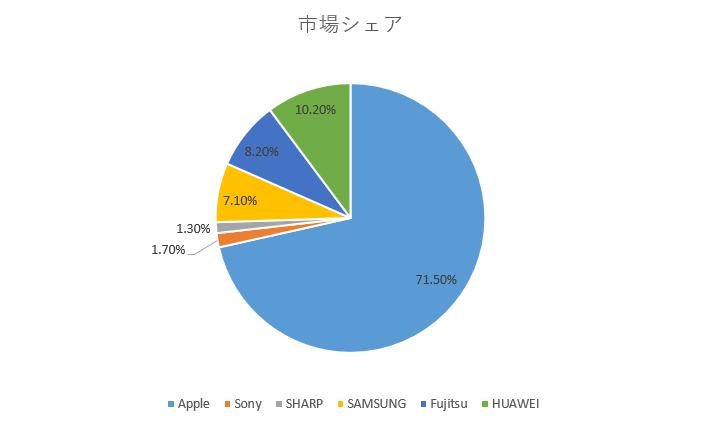
\includegraphics[width=15cm]{share.jpg}
	\caption{市場シェア率}
\end{figure}	


\section{広告効果の最適化}
多変数の最適化は数学的に困難である。
そこで広告費の割り当てを整数の離散値として総当たりで求める。

\begin{lstlisting}[caption=広告費用の離散最適化, frame=single, language=python]
results = []
sets = []
for a in range(201):
    for b in range(201-a):
        for c in range(201-a-b):
            d = 200 - (a+b+c)
            result = product_data.loc['AQUOS R2','ios']*a*0.329605
            	+ product_data.loc['AQUOS R2','RAM']*b*(-0.244887)
            	+ product_data.loc['AQUOS R2','out_camera']*c*(-0.19905)
            	+ product_data.loc['AQUOS R2','width']*d*(-0.19765)
            results.append(result)
            sets.append([a, b, c, d])
            
m_result = max(results)

for i, result in enumerate(results):
    if result == m_result:
        print(i)
 
 #output: 20300
        
sets[20300]
# [0, 200, 0, 0]
\end{lstlisting}

最適化した広告費を市場に適応させる。
理解度についてのテーブルを変更する。

\begin{lstlisting}[caption=広告費を変更した各製品の属性ごとの理解度, frame=single, language=python]
marketing = pd.DataFrame([[50, 50, 50, 50]
                          , [50, 50, 50, 50]
                          , [0, 200, 0, 0]
                          , [50, 50, 50, 50]
                          , [50, 50, 50, 50]
                          , [50, 50, 50, 50]
                          ]
                         , columns = ['ios', 'RAM', 'out_camera', 'width']
                         , index= ['Apple', 'Sony', 'SHARP',
                              'SAMSUNG', 'Fujitsu', 'HUAWEI']
                        )
effect_of_marketing = []
for i, name in enumerate(marketing.index):
    for j, column in enumerate(marketing.columns):
        effect_of_marketing.append(np.random.normal(
                loc = ad_effect(marketing.iloc[i, j])
                                       , scale = 0.1
                                       , size = 1000
                                       )
                      
                  )
effect_of_marketing = np.array(effect_of_marketing)
pd.DataFrame(effect_of_marketing).T.to_csv("effect_change.csv")
\end{lstlisting}

この結果が以下のグラフである。
\begin{figure}[H]
	\centering
	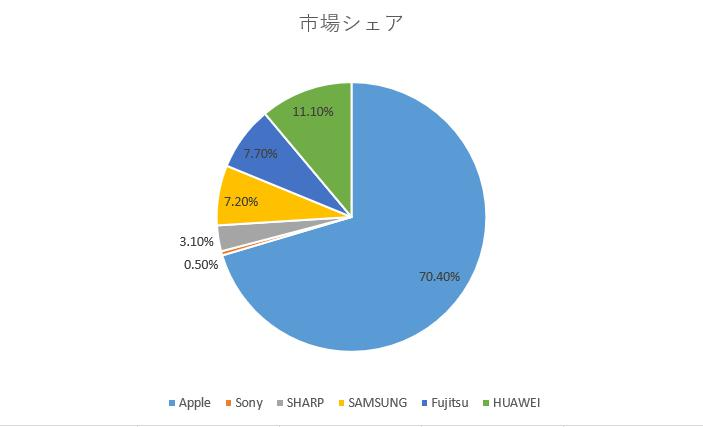
\includegraphics[width=15cm]{share_change.jpg}
	\caption{広告費用変更後の市場シェア率}
\end{figure}

\section{考察}
はっきり言えば広告費を最適化したところでシェア率が大幅に上昇することはなかった。
これはiosの人気が高いにもかかわらず、その他の属性値でiPhoneとの差別化ができていないことに起因する。
逆に属性値の似通ったSonyのXperiaのシェアは広告費の変更によって奪うことができた。

顧客の属性値のscaleを大きくしている為、ニッチ層が多くできたこともSHARPがシェアを取れなかったことの原因の一つである。
特にHUAWEIはiPhoneとは逆にカメラの画素数を上げ、RAMを多く積んでいる。
比較的大きな分散で画素数やRAMの高スペックを望む層について顧客を確実に獲得している。

なぜかiPhoneが日本では圧倒的なシェアを誇ってしまっているのでその傾向に引きずられている。
iPhoneと似通うと顧客の満足度には近づくが、iPhoneに負ける為購入に至らないケースが大かった。

スマートフォン等の電子機器を始め、比較的高額な商品は消費者も吟味して一番良いと思ったものを買うためその顧客にとって1番でなければシェアが取れないことを痛感した。

\section{今後の課題}
\begin{itemize}
\item 市場自体を動かしてiosからシェアを奪うにはどうすればよいか。
\item Androidの中でシェアを獲得するにはどうしたらいいだろうか。
\item 製品改良はどこを重視していけばよいだろうか。
\item 顧客が求める商品像とは。
\item 標準偏差は正しかっただろうか
\end{itemize}

% 参考文献 \cite{}で表示
\begin{thebibliography}{99}
	\bibitem{a} docomo \url{https://www.nttdocomo.co.jp/product/?icid=CRP_TOP_to_CRP_PRD}
	\bibitem{b}デジマライフ iphoneバッテリー容量比較 \url{https://digimamalife.com/iphone-ipad-battery-size}
	\bibitem{c} ITmedia Mobile \url{http://www.itmedia.co.jp/mobile/articles/1805/11/news133.html}
	\bibitem{e} 株式会社ウェブレッジ
	\bibitem{d} Pythonでデータサイエンス \url{https://pythondatascience.plavox.info/scikit-learn/%E7%B7%9A%E5%BD%A2%E5%9B%9E%E5%B8%B0}
\end{thebibliography}


\end{document}

%チートTips
\begin{comment}
%画像貼り付け   [H]で場所固定
\begin{figure}[H]
	\centering
	\includegraphics[width=15cm]{hoge.png}
	\caption{figure-hoge}
\end{figure}


%コードの挿入
\begin{lstlisting}[caption=課題1, frame=single, language=python]

\end{lstlisting}

%表
\begin{table}[H]
\centering
\caption{table hoge}
  \begin{tabular}{l|crr}
    メニュー & サイズ & 値段 & カロリー \\
    牛丼 & 並盛 & 500円 & 600 kcal \\
    牛丼 & 大盛 & 1,000円 & 800 kcal \\
    牛丼 & 特盛 & 1,500円 & 1,000 kcal \\
    牛皿 & 並盛 & 300円 & 250 kcal \\
    牛皿 & 大盛 & 700円 & 300 kcal \\
    牛皿 & 特盛 & 1,000円 & 350 kcal
  \end{tabular}
\end{table}

%url
\url{}

\end{comment}
